\section{definition14-2(intergenerator move)}
\begin{definition}
\end{definition}

Suppose we have an inter-generator diagram on $n$ strands. Then we define a collection of moves, called inter-generator move, inductively so that the final diagram looks as follows:

\begin{figure}[H] % Optional: [h] means here, [t] for top, [b] for bottom, [p] for page of floats
    \centering
    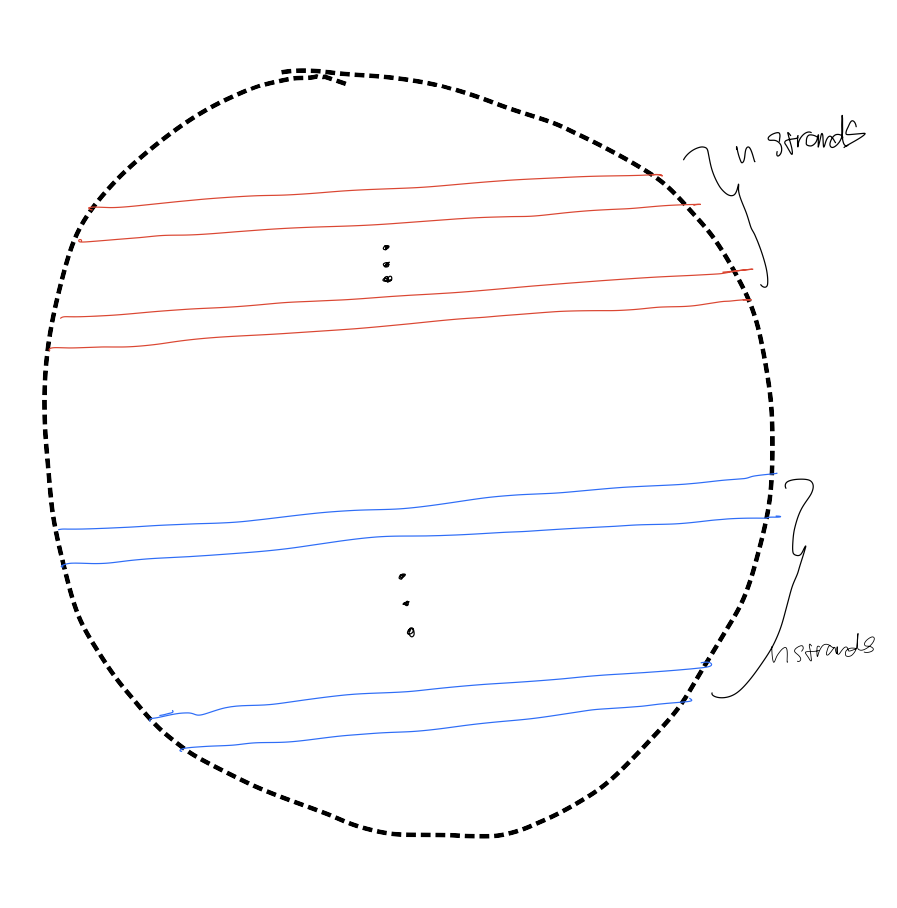
\includegraphics[width=\linewidth]{diagrams/definition14-2/1.png} % Adjust the width as needed
    \caption{Your caption here}
    \label{fig:your-label}
\end{figure}

If $n=1$, then intergenerator move is the null move. Suppose $n > 1$ and we have defined intergenerator move up to $n-1$ strands. Suppose we have the following inter-generator diagram on $n$ strands :

\begin{figure}[H] % Optional: [h] means here, [t] for top, [b] for bottom, [p] for page of floats
    \centering
    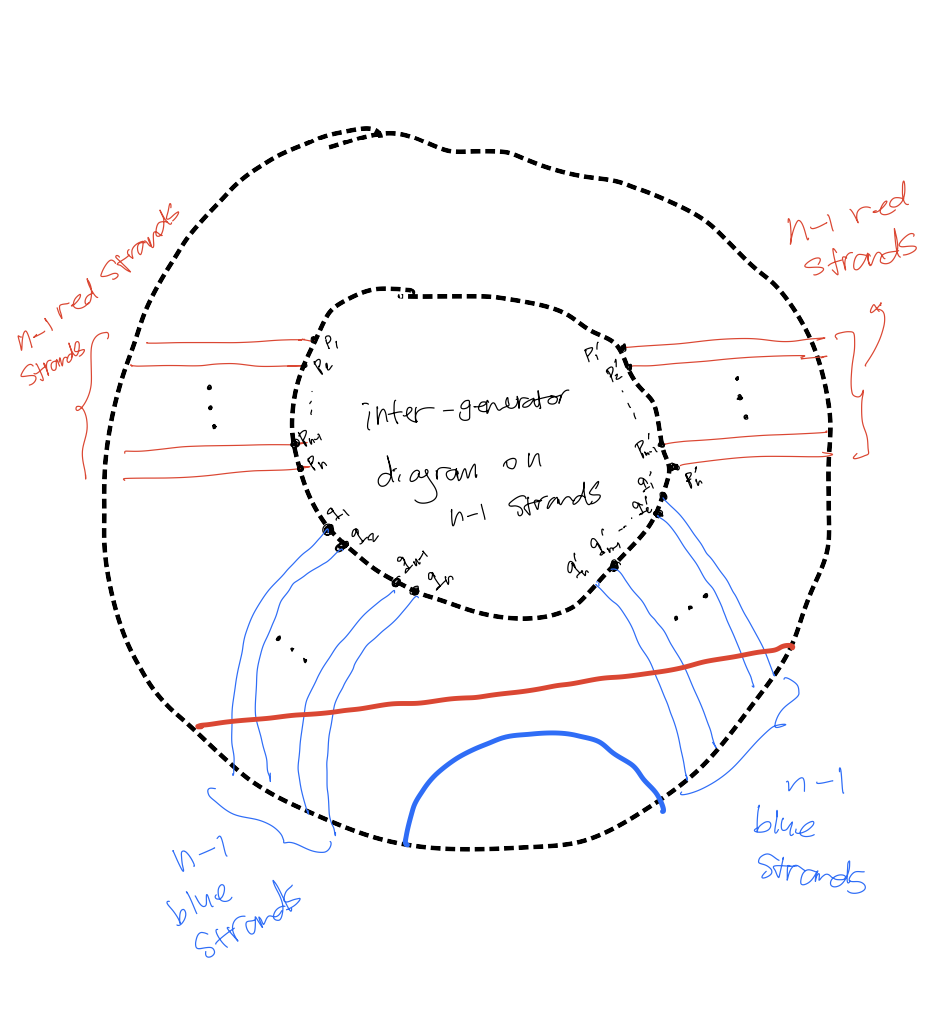
\includegraphics[width=\linewidth]{diagrams/definition14-2/2.png} % Adjust the width as needed
    \caption{Your caption here}
    \label{fig:your-label}
\end{figure}

(Step1) Apply intergenerator move to the intergenerator diagram on $n-1$ strands inside the smaller disk we get

\begin{figure}[H] % Optional: [h] means here, [t] for top, [b] for bottom, [p] for page of floats
    \centering
    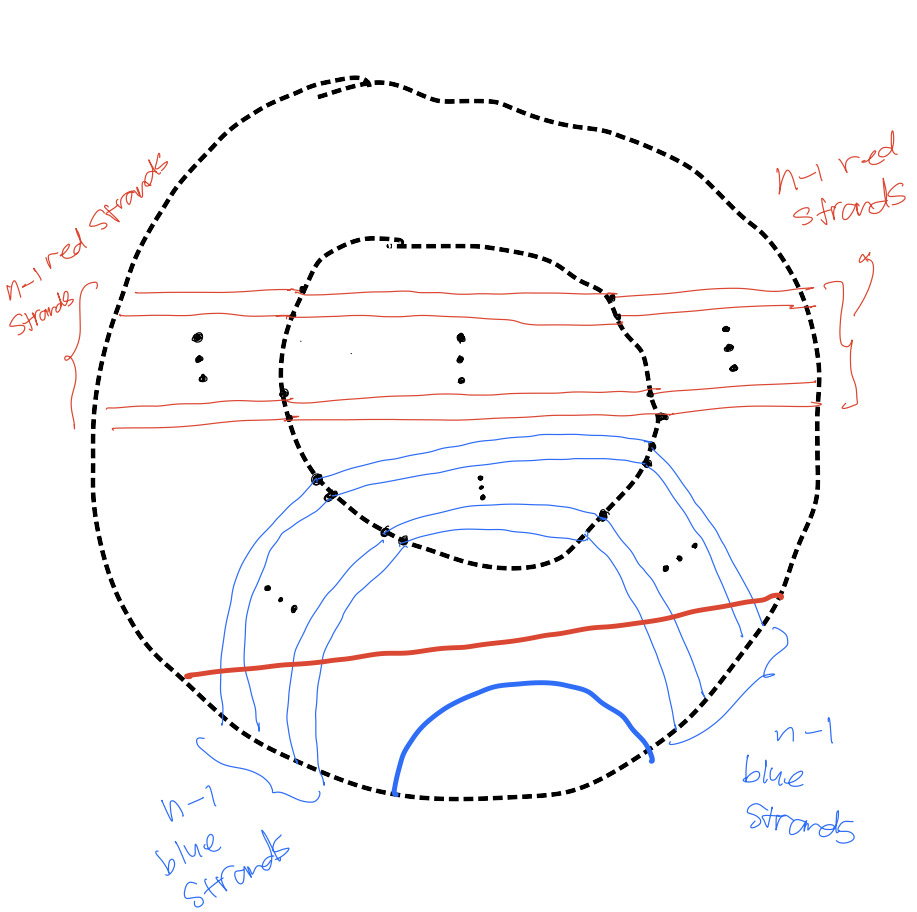
\includegraphics[width=\linewidth]{diagrams/definition14-2/3.png} % Adjust the width as needed
    \caption{Your caption here}
    \label{fig:your-label}
\end{figure}

(Step2) Apply MOVE \RN{6}(successive application of reverse Reidemeister moves) inside the region surrounded by the purple circle

\begin{figure}[H] % Optional: [h] means here, [t] for top, [b] for bottom, [p] for page of floats
    \centering
    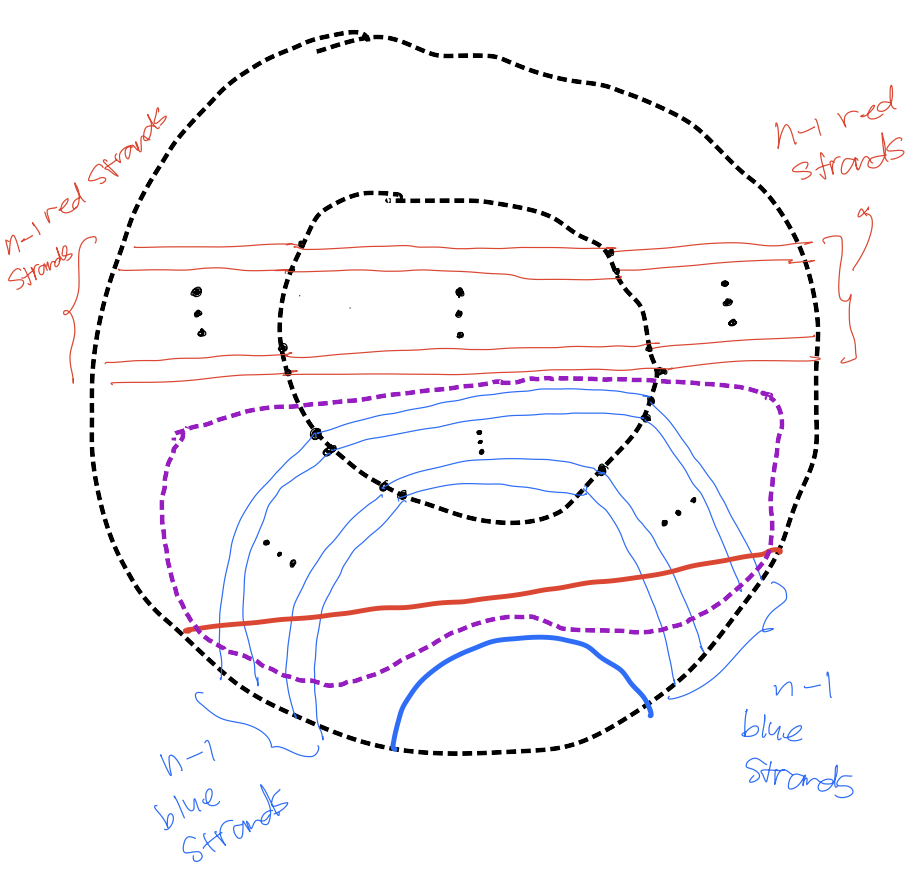
\includegraphics[width=\linewidth]{diagrams/definition14-2/4.png} % Adjust the width as needed
    \caption{Your caption here}
    \label{fig:your-label}
\end{figure}

we get :

\begin{figure}[H] % Optional: [h] means here, [t] for top, [b] for bottom, [p] for page of floats
    \centering
    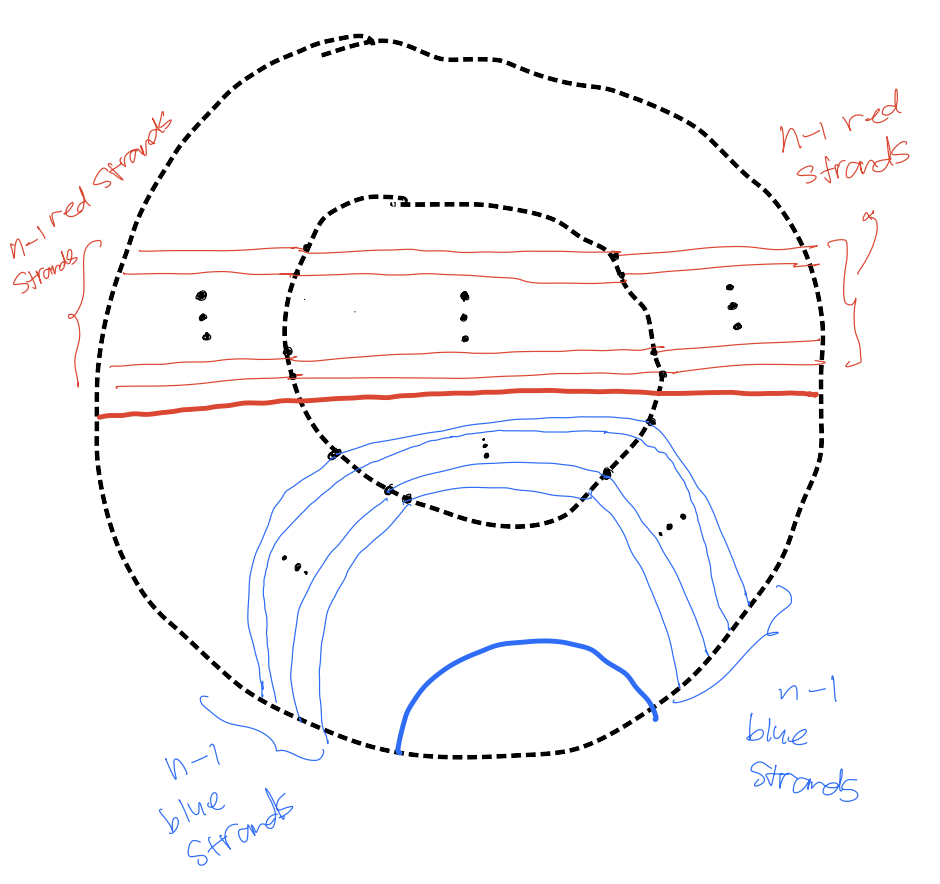
\includegraphics[width=\linewidth]{diagrams/definition14-2/5.png} % Adjust the width as needed
    \caption{Your caption here}
    \label{fig:your-label}
\end{figure}